%!TEX program = xelatex
% 完整编译: xelatex -> bibtex -> xelatex -> xelatex
\documentclass[lang=cn,11pt,a4paper,cite=authoryear]{elegantpaper}
\usepackage{algorithm}
\usepackage{algpseudocode}
\usepackage{algorithmicx}
\usepackage{pdfpages}
\title{经典力学体系下多体问题的模拟与并行优化}
\author{陈实 \\ 华东理工大学}
%\version{0.02}
\date{\zhtoday}

\usepackage{array}
\usepackage{amsmath}
\floatname{algorithm}{算法}
\renewcommand{\algorithmicrequire}{\textbf{输入:}}
\renewcommand{\algorithmicensure}{\textbf{输出:}}
\newcommand{\ccr}[1]{\makecell{{\color{#1}\rule{1cm}{1cm}}}}

\begin{document}

%\includepdf[pages={1}]{preface.pdf} 

\maketitle

\begin{abstract}

多体问题又被称为$N$体问题$(N>0)$,是一般力学与天体物理学的基本问题之一,其研究的是$N$个质点在万有引力作用下的运动规律。多体问题有着广泛的应用场景,既能用于探索天体物理学中宇宙星体的演化与相互作用,又能用于研究分子动力学中分子、原子等微观粒子的运动规律。然而,若使用以经典力学为理论基础的模拟法对这一问题进行求解,由于需要计算每个质点对之间的相互作用,其时间复杂度高达$\text O(N^2)$,这对动辄千万数量级的模拟实验来说十分难以接受。因此,许多学者纷纷探索了以牺牲一定运算精度为前提的优化算法。在这其中最具代表意义的,是最早由Barnes和Hut在1986年提出的一种以$k$维树为基础的方法,这一方法能够将计算过程的时间复杂度降低至$\text O(N\log N)$,使得多体问题的模拟规模上限得到了巨大的提升。

鉴于此,本文首先描述了多体问题的朴素模拟法,随后阐述了如何使用MPI框架对其进行并行优化。接着,本文介绍了一种以Barnes和Hut提出的方法为原型,以$k$维树\footnote{为便于说明,本文所示代码与示意图均针对于二维平面上的多体问题,在实现时采用了四叉树数据结构。具体的算法实现和并行优化方法都可以方便地推广到三维空间。}为基础的多体模拟的高效实现\footnote{本文所使用的代码和数据均可从 \href{https://github.com/PHIKN1GHT/n_body_simulation}{Github::N\_body\_simulation} 获取。},并尝试使用OpenMP框架对其进行并行优化。以上工作综合运用了笔者在高性能计算课程中所学的相关知识,并为多体问题的模拟与并行优化研究提供了一定的基础。

\keywords{多体模拟,四叉树,并行计算,MPI,OpenMP}
\end{abstract}

\newpage

\section{绪论}

\subsection{课题背景}

首先回顾一下$N$体问题的发展史:$N$体问题是一个用于描述在牛顿运动定律下N个质点的运动的常微分方程组,除去$N=1$的平凡情况,在$N=2$时,该问题退化为开普勒问题,有着确定的解:当我们将一个质点固定于原点时,另一个质点的运动轨迹将会是一个圆锥曲线——包括圆、椭圆、抛物线和双曲线。对于$N>2$的广义$N$体问题,目前普遍认为无法求出解析解\footnote{庞加莱在他的著作《天体力学新方法》中指出,可以找出一定限制下多体问题具有周期性的解析解。}。

尽管广义$N$体问题无法求解,我们可以通过数值积分方式对特定初态的发展过程进行模拟。常见的模拟方法有朴素模拟法与网格化法。前者直接计算每个质点对于其它所有质点的受力之和,因而时间复杂度高达$\text O(N^2)$。网格化法将整个空间划分为网格,把质点折算到其位置附近的格点之上,降低了时间复杂度,但由于网格划分尺度一定,对于距离较近的质点来说误差较大。基于k维树的Barnes-Hut方法实质上可以看作是一个改进的网格化方法,其通过限制按格点近似计算受力的距离的最小值,并按照质点分布的疏密动态划分网格,使得时间复杂度保持在$\text O(N\log N)$的情况下,降低了近距离质点之间的计算误差,并在实际应用中获得了较好的结果。

在实际工程中,除去以上基本算法之外,常见的还有着一些混合算法与近似算法,前者包括粒子-网格算法、Batnes-Hut-网格算法等,后者包括FMM算法、Anderson算法等。

\subsection{形式化表述}

考虑在牛顿参考系$\mathbf R^3$中运动的$N$个质点,其之间的相互作用只有万有引力。假设第$i$个质点具有位置矢量$\mathbf q_i$,且质量$m_i>0$,那么由牛顿第二定律和引力定律,第$i$个质点的运动方程为:
\[
m_i\mathbf{\ddot{q_i}}=\sum_{j=1}^N \frac{Gm_im_j(\mathbf{q_j}-\mathbf{q_i})}{||\mathbf{q_i}-\mathbf{q_j}||^3}
\]
上式也被称为$N$体问题的牛顿公式。该式中,$G$是万有引力常数,圆点$\cdot$表示对$t$求导,也即$\cdot\cdot=\mathrm {d^2/dt^2}$,且我们约定$i=j$项可从总和中略去。

尽管爱因斯坦相对论方程可以为多体问题提供更准确的表述,但工程经验表明上式已经足够有效\footnote{足以使得人们登上月球,并把探测器送至火星。},且爱因斯坦相对论方程难以进行数值求解,因此不作进一步展开。同理,$N$体问题的哈密顿公式由于与后文的算法实现无关,在此也不作陈述。

\subsection{并行系统选用}

在实际应用中,多体模拟的问题规模达到了千万级别以上,对浮点运算的需求也多达数十乃至数百TFlops,因而一般个人家用计算机或是单处理机已经难以求解这一问题,需要使用较复杂的并行系统来进行高性能计算。

常见的并行系统包括:并行向量处理机、对称多处理机、大规模并行处理机与工作站集群,其中对称多处理机与工作站集群因为较好的效益成本比已经逐渐成为主流。

本文主要研究了多体模拟的朴素算法与k维树算法的并行优化方法:前者的实现基于MPI框架,采用了非远程存储访问模型,可运行于工作站集群;后者的实现基于OpenMP框架,采用了均匀存储访问模型,可运行于对称多处理机。

\begin{figure}[htbp]
  \centering
  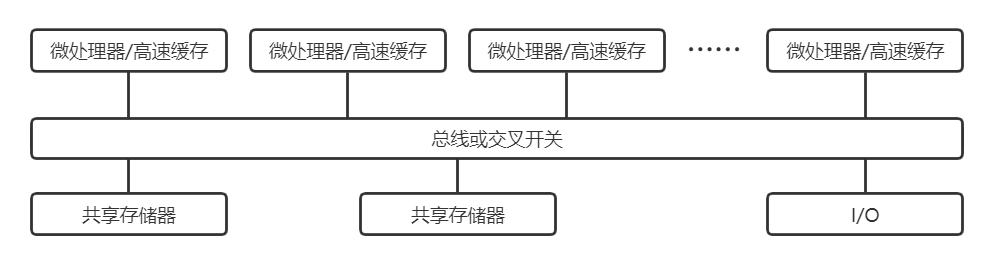
\includegraphics[width=\textwidth]{SMP.png}
  \caption{对称多处理机结构模型}
\end{figure}

\newpage

\section{朴素算法}

朴素算法即指直接按照牛顿公式进行数值积分运算来求解各个质点运动轨迹的方法。具体来说,不失一般性,我们定义每个质点$p_i$有位置矢量$\mathbf q_i=\{x_i,y_i\}$、速度矢量$\mathbf v_i=\{vx_i,vy_i\}$与质量$m_i$,并定义质点数量$N$为某一正整数,时间步长$\mathrm dt$为一足够小的正实数,$G$为万有引力常数,那么可直接根据牛顿公式计算出每个点的受力情况\footnote{在实现过程中,为避免出现数值异常,需要考虑对过近的距离进行软化。为便于研究,本文在实现时直接将最短距离设为常值。关于距离软化函数在工程中的常见实现可参阅\cite{en1}。},进而计算出其速度矢量和位置矢量的增量。

尽管朴素算法时间复杂度较高,在多体问题的求解中,其目前依然是精度最高\footnote{仅在经典力学体系下,也即不考虑爱因斯坦相对论方程的情况下。}的算法,因而具有一定的实际意义。

\subsection{朴素算法的代码实现}

见图例。

\begin{figure}[htbp]
  \centering
  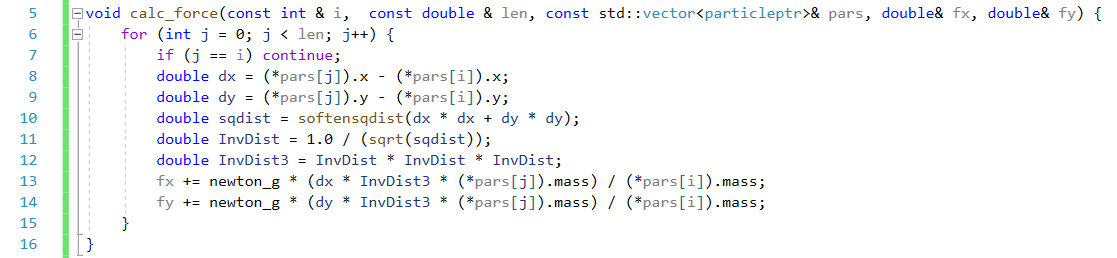
\includegraphics[width=\textwidth]{bruteforce_calc_force.png}
  \caption{求解受力过程,节选自[bruteforce.cpp]}
\end{figure}

\begin{figure}[htbp]
  \centering
  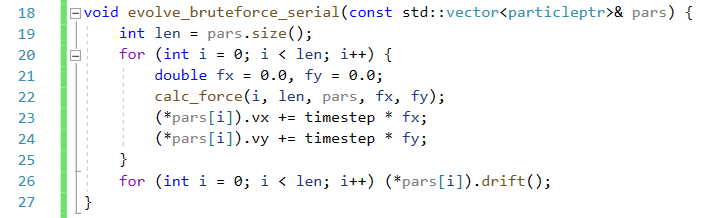
\includegraphics[width=\textwidth]{bruteforce_serial.png}
  \caption{朴素算法的串行实现,节选自[bruteforce.cpp]}
\end{figure}

\subsection{朴素算法的并行优化}

接下来考虑这一算法的并行优化:首先我们观察到该算法可以被很自然地划分为两个阶段:受力分析阶段与位移结算阶段。在受力分析阶段,计算出每个点受其它点的作用力之和,在位移结算阶段,将受力乘以时间步从而得到了位移的增量,进而更新每个结点的位移增量。

这两个阶段之间存在依赖关系,但在每个阶段之内,每个质点的运算结果与其它结点的运算结果之间并不存在数据依赖冲突,因此可以直接用划分设计技术对原问题进行分解,从而实现并行化。

具体来说,考虑$p$个处理器的情况,在每个阶段将规模为$N$的问题划分为$p$个规模为$\lceil  \frac{N}{p}\rceil$的子问题,然后将子问题分配到每个处理器上分别求解。求解完成后,所有处理起再将数据发给某个处理器$p_0$,$p_0$将求解结果整合后再反馈给各个处理器,随后进入下一阶段\footnote{实际实现中,受时间所限,笔者只对耗时占比较大的第一阶段进行了并行优化。}。

\subsection{朴素算法并行优化的代码实现}

\begin{figure}[htbp]
  \centering
  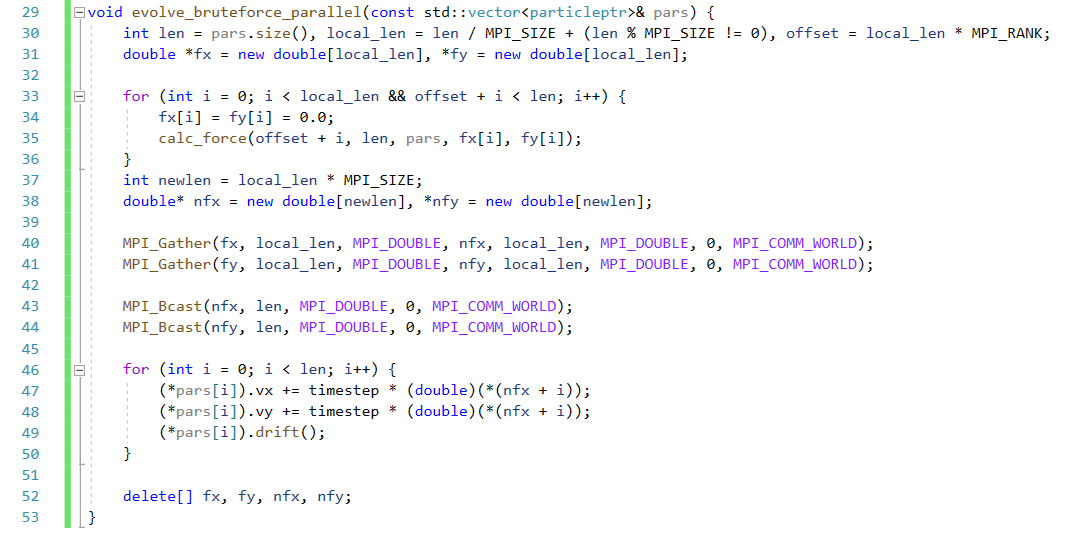
\includegraphics[width=\textwidth]{bruteforce_parallel.png}
  \caption{朴素算法的并行实现,节选自[bruteforce.cpp]}
\end{figure}

\newpage

\section{$k$维树算法}

多体模拟问题的$k$维树算法又称Barnes-Hut算法,其原理是利用$k$维树的高效索引能力,将某些远距离的质点的作用力的转化为对某个格点(也即$k$维树的某个结点)的作用力,因而减少了求解过程的计算量。

\begin{figure}[htbp]
  \centering
  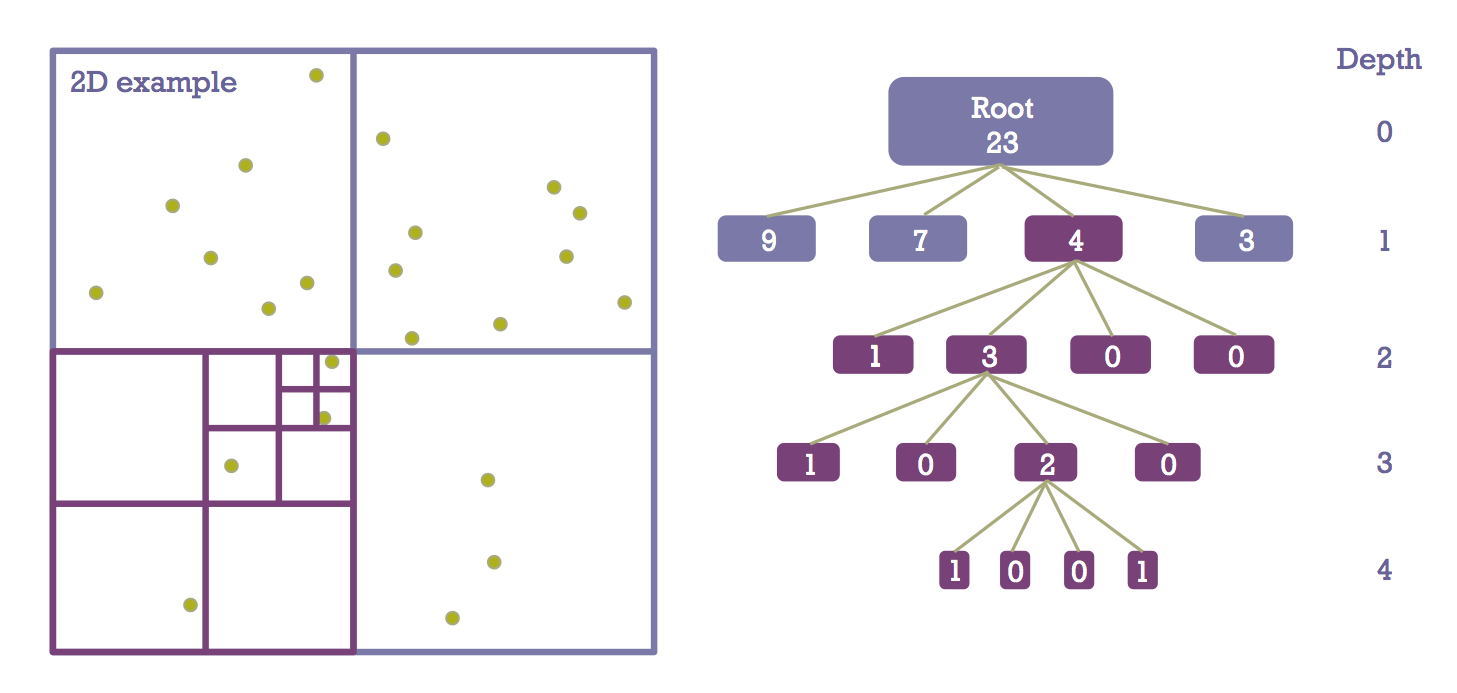
\includegraphics[width=\textwidth]{Barnes-Hut_tree.png}
  \caption{Barnes-Hut算法的示意图,引用自\href{http://portillo.ca/nbody/barnes-hut/}{portillo.ca}}
\end{figure}

对$k$维树实现细节的论述并非本文重点,因而不在此进行赘述。为简化研究对象,本文主要实现了一种确定划分\footnote{实际工程中需要选用某种策略估算出质点分布的中心,出于简化目的,本文在实现时假定质点分布始终围绕着原点也即$\{0,0\}$。}的四叉树。具体实现方式可以参阅项目中的代码文件[quadtree.h]。

\subsection{$k$维树算法的代码实现}

见图例。此处主要展示的是简化了的利用四叉树进行。

\begin{figure}[htbp]
  \centering
  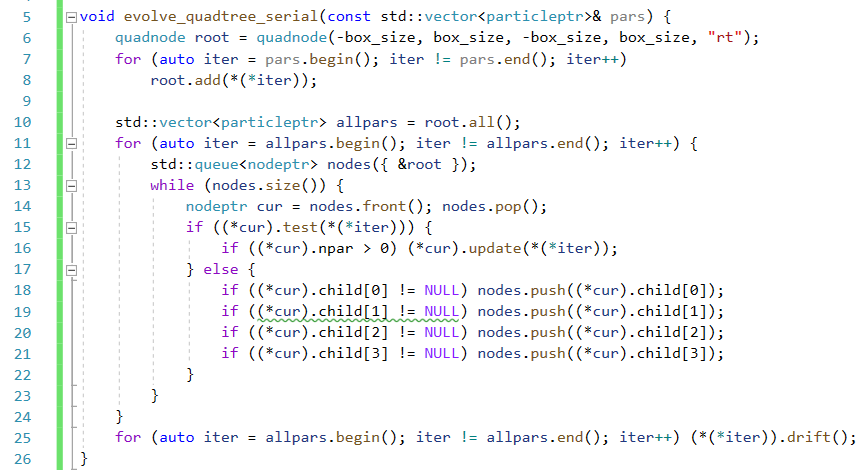
\includegraphics[width=\textwidth]{quadtree_serial.png}
  \caption{$k$维树算法的串行实现,节选自[quadtree.cpp]}
\end{figure}

\subsection{$k$维树算法的并行优化}

相较于朴素算法,$k$维树算法的并行优化要较复杂一些,但也依然符合对树型结构进行并行化设计的通用方法。总体来说,对树型结构进行并行化有两大思路:层级并行化(或称广度优先并行化)与子树并行化(或称深度优先并行化)。

\begin{figure}[htbp]
  \centering
  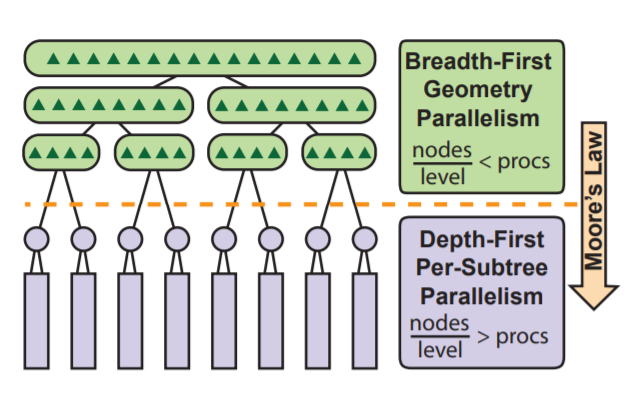
\includegraphics[width=\textwidth]{parallel_tree_design.png}
  \caption{层级并行化与子树并行化及其适应情况的示意图,引用自\cite{en2}}
\end{figure}

层级并行化指将当前层级的每个结点分配给一个处理机,这种并行优化方式实现起来较为简单,且比较符合直觉;而子树并行化则是指在树的某一层开始不再将下层进行并行划分,转而让当前处理机完全负责该子树的所有运算。总体来说,这两种并行思路各有优劣,也都有着自己的使用场景。层级并行化使得处理机之间的通信比较频繁,因而适合当前深度的宽度(即结点总数)与处理机个数相比较小或持平的情况;而子树并行化与之恰好相反,单个线程要处理的任务较多,因而适合宽度远大于处理机个数的情况。

那么,对于$k$维树算法的具体并行优化方法就呼之欲出了:由于本文中实现的$k$维树简化了划分过程\footnote{在实际工程中,$k$维树的划分过程往往需要一个确定划分点的启发式策略。常用的思路是将所有质点在各个维度上进行排序后再选取中点作为划分点,这就涉及到了并行排序算法设计的问题。本文实现的$k$维树为了便于研究,直接选用中点作为划分点,简化了这一过程。},因而难点主要在子树构建。子树的构建过程是自顶向下(也就自根结点向叶子结点)使用递归实现的,考虑直接根据某一层的宽度进行两种不同的并行化设计,会发现直接求本层宽度的开销比较大,但在测试时,生成的质点又是随机分布的,那么可以考虑一个简单的近似方法:直接为层级并行化所允许的深度设一个上限,若深度超过该上限,并行过程停止,转为串行(也即从该层开始使用子树并行化设计)。

\subsection{$k$维树算法并行优化的代码实现}

见图例。

\begin{figure}[htbp]
  \centering
  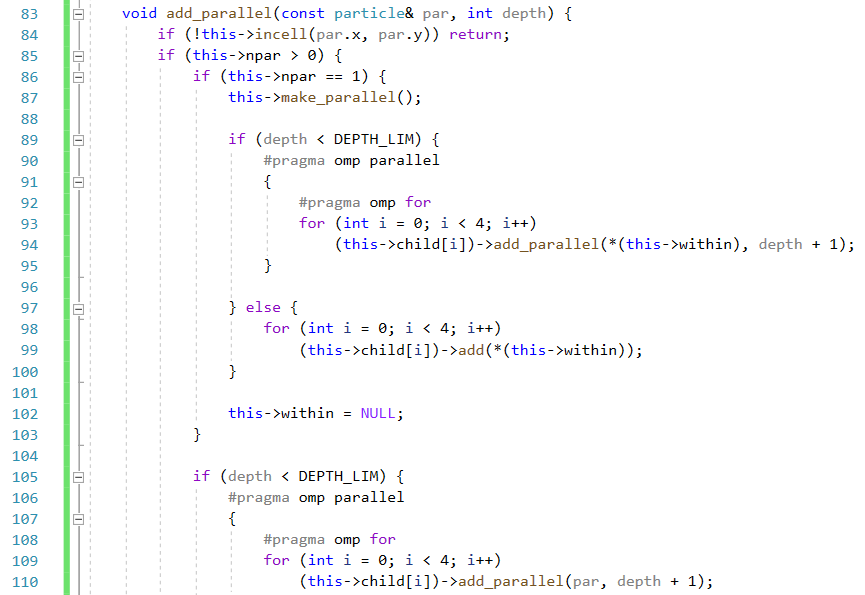
\includegraphics[width=\textwidth]{add_parallel_1.png}
  \caption{$k$维树算法中子树构建算法的并行实现(上),节选自[quadtree.h]}
\end{figure}

\begin{figure}[htbp]
  \centering
  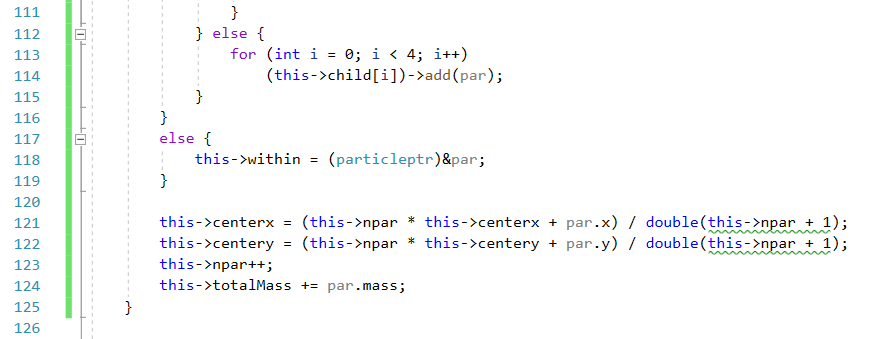
\includegraphics[width=\textwidth]{add_parallel_2.png}
  \caption{$k$维树算法中子树构建算法的并行实现(下),节选自[quadtree.h]}
\end{figure}

\begin{figure}[htbp]
  \centering
  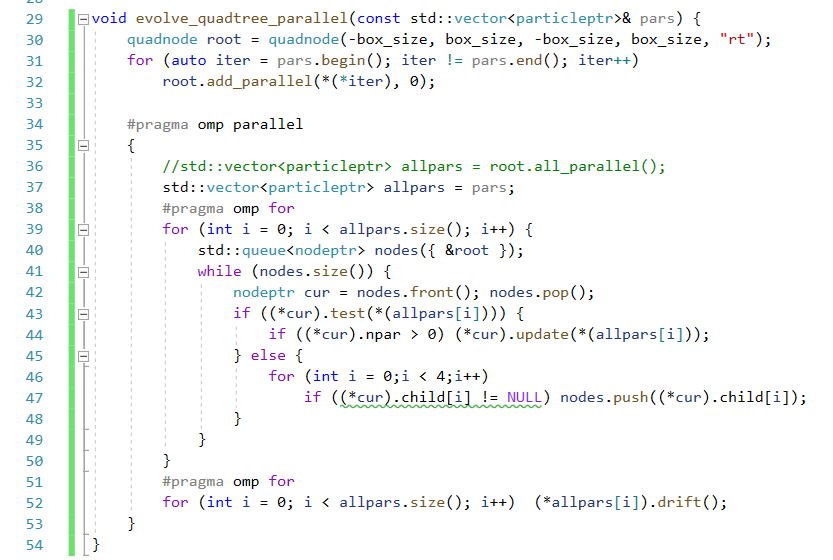
\includegraphics[width=\textwidth]{quadtree_parallel.png}
  \caption{$k$维树算法的并行实现,节选自[quadtree.cpp]}
\end{figure}

\newpage

\section{相关实验}

\subsection{实验环境}
\begin{itemize}
\item 处理机:Intel Core i5-8265U 4C8T
\item 内存容量:16.0G
\item 操作系统:Windows 10 Home x64
\item 编译器:MSVC 14.25.28610 (/o2\footnote{即开启编译选项 Maximum Optimization (Favor Speed)。})
\end{itemize}

\subsection{验证时间复杂度}

首先对这两个算法的时间复杂度进行验证:随机生成$N=\{256,512,1024,2048,4096,8192,16384\}$个均匀分布在空间中的质点,分别代入朴素算法$k$维树算法并记录求解所用时间。结果见图例。

\begin{figure}[htbp]
  \centering
  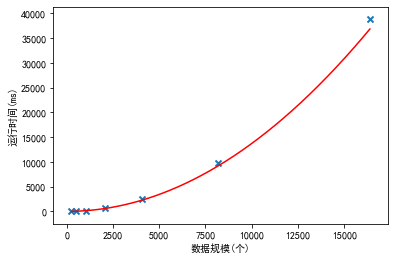
\includegraphics[width=12cm]{exp_1.png}
  \caption{朴素算法的时间复杂度拟合结果,图中红色曲线为$O(N^2)$}
\end{figure}

\begin{figure}[htbp]
  \centering
  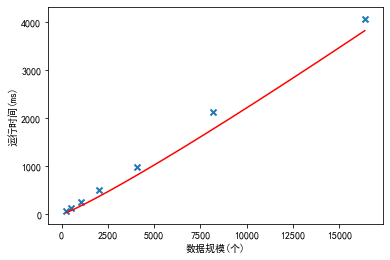
\includegraphics[width=12cm]{exp_2.png}
  \caption{$k$维树的时间复杂度拟合结果,图中红色曲线为$O(N\log N)$}
\end{figure}

\newpage
\subsection{测试加速比}

结果见图例。

\begin{figure}[htbp]
  \centering
  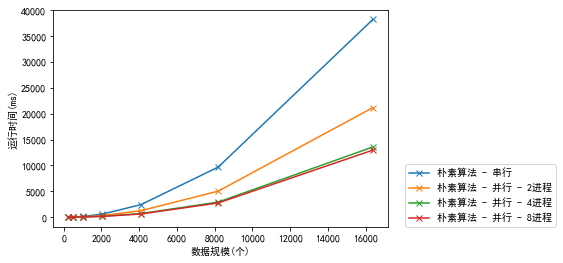
\includegraphics[width=\textwidth]{exp_3.png}
  \caption{朴素算法的并行优化在多处理机下的执行时间}
\end{figure}

\begin{figure}[htbp]
  \centering
  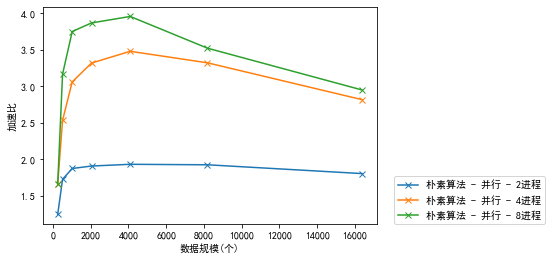
\includegraphics[width=\textwidth]{exp_5.png}
  \caption{朴素算法的并行优化在多处理机下的加速比}
\end{figure}

\begin{figure}[htbp]
  \centering
  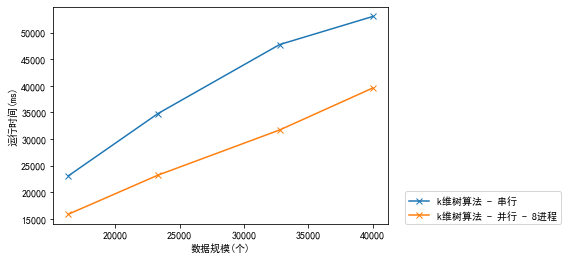
\includegraphics[width=\textwidth]{exp_4.png}
  \caption{$k$维树算法的并行优化在多处理机下的执行时间}
\end{figure}

\begin{figure}[htbp]
  \centering
  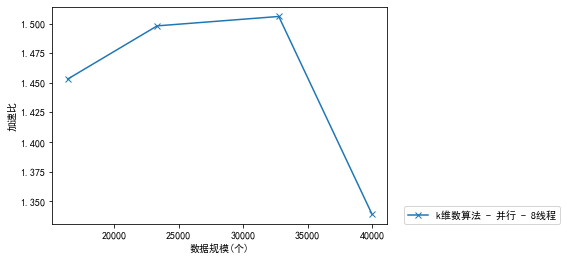
\includegraphics[width=\textwidth]{exp_6.png}
  \caption{$k$维树算法的并行优化在多处理机下的加速比}
\end{figure}

\newpage
\subsection{实验结果可视化}

结果见图例。

\begin{figure}[htbp]
  \centering
  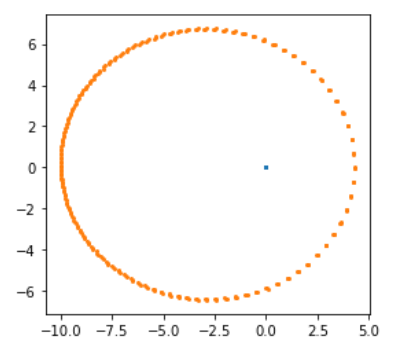
\includegraphics[width=6cm]{example1.png}
  \caption{测试样例1:开普勒问题,基于$k$维树}
\end{figure}

\begin{figure}[htbp]
  \centering
  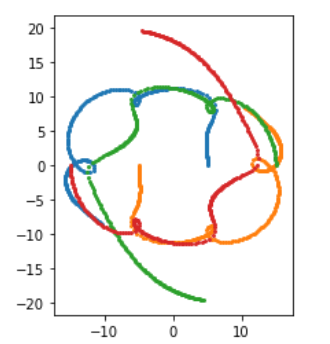
\includegraphics[width=6cm]{example2.png}
  \caption{测试样例2:对偶开普勒问题,基于$k$维树}
\end{figure}

\newpage
\section{结论}

受时间所限,本文仅分析了求解多体问题的朴素算法和$k$维树算法的一种简单实现
\footnote{本文中的实现忽略了划分点的选取、$k$维树的平衡状态的维护等较复杂的内容。},并针对其分别设计了并行优化方案,随后对结果进行了测试。

单从已有结果来看,朴素算法的并行优化最高$3.9$的加速比还是比较令人满意的,但$k$维树算法的加速比最高仅有$1.5$\footnote{笔者对算法中的超参数进行过搜索,暂未发现更好的结果。},其实并不能算是非常成功的并行优化。究其原因,笔者认为可能和在实现串行$k$维树时所选用的数据结构或实现逻辑有关。

事实上,也曾有许多学者提出过关于$k$维树构建过程与平衡过程的并行优化方案。限于时限与篇幅,笔者没有在此进行过多的研究与实验。 

希望本文能为多体问题的模拟与并行优化研究提供一些基础。

\section{致谢}

感谢科幻文学作家刘慈欣,其著名作品《三体》是本文灵感的来源之一。

感谢孙宇飞同学,用专业的物理知识即时阻止了我妄图以对爱因斯坦相对论方程进行数值求解作为本文切入点的意图。

感谢丁锐同学,协助我理清了$k$维树并行优化方案的诸多关键步骤。

\nocite{*}
\bibliography{refers}

\end{document}
